\documentclass[a4paper, 12pt]{article}

%\usepackage{cmap}
\usepackage[T2A]{fontenc}
\usepackage[utf8]{inputenc}
\usepackage[english, russian]{babel}
\usepackage{graphicx}
\usepackage[top=1in, bottom=1in, left=3.2cm, right=2.6cm]{geometry}
\graphicspath{./}
\usepackage{biblatex}
\addbibresource{lib.bib}
\linespread{1.5}
\usepackage{ragged2e}
\justifying
\usepackage{listings}
\usepackage{color}


\begin{document}
	
\begin{titlepage}
	\fontsize{12pt}{12pt}\selectfont
	\begin{figure}[t!]
		\centering
		
\includegraphics[scale=0.8]{bmstu}
	\end{figure}
	
	\noindent\rule{15cm}{3pt}
	\newline\newline
	\noindent 
	ФАКУЛЬТЕТ 
	\underline{«Информатика и системы управления»} \newline\newline
	
	\noindent КАФЕДРА \underline{«Программное обеспечение ЭВМ и информационные технологии»}\newline\newline\newline\newline\newline
	
	\centering {\Large Отчет по лабораторной работе № 1}
	\vspace{1mm}
	
	\centering {\Large По курсу: "Функциональное и логическое программирование"
		\vspace{8mm}	
		
		\centering \bf Списки в Lisp. Использование стандартных функций.}
	\vspace{8mm}
	
	
	\begin{flushright}
		{\small	Студент:\\ Турсунов Жасурбек Рустамович \\ Группа: ИУ7-56Б
			\vspace{3mm}
			\\Преподователи: \\ Толпинская Наталья Борисовна \\ Строганов Юрий Владимирович}
	\end{flushright}
	
	\begin{center}
		\vfill
		Москва, \the\year
		~г.
	\end{center}
\end{titlepage}

\tableofcontents
\clearpage
\newpage

\textbf{Цель работы:} приобрести навыки использования списков и стандартных функций Lisp.
\\ \hspace*{5mm} \textbf{Задачи работы:} изучить способ использования списков для фиксации информации, внутреннее представление одноуровневых и структурированных списков, методы их обработки с использованием базовых функций Lisp.


\section*{Введение}
\addcontentsline{toc}{section}{Введение}


	\hspace*{5mm} Функциональное программирование ориентировано на символьную обработку данных. Предпологается, что любую информацию можно свести к символьной. Слово <<символ>> здесь близко к понятию <<идентификатор>>.
	\\ Базис Lisp образуют:
	\begin{enumerate}
		\item атомы;
		\item структуры;
		\item базовые функции;
		\item базовые функционалы.
	\end{enumerate}
	\textbf{Символьное выражение} это атом или точечная пара.
	\\ \textbf{Атомами являются:} 
	\begin{enumerate}
		\item \textbf{символы(идентификаторы)} - синтаксически - набор литер(букв латинского алфавита и цифр), начинающихся с буквы;
		\item \textbf{специальные символы - {T, Nil}} - используются для обозначения <<логических констант>>;
		\item \textbf{самоопределимые атомы} - натуральные числа, дробные числа, вещественные числа, строки - последовательность символов, заключенных в двойные апострофы.
	\end{enumerate}
	\hspace*{5mm} Более сложные данные в Lisp выстраиваются с помощью \textit{бинарных узлов}, содержащих пару указателей. Каждый бинарный узел соответствует минимальному блоку памяти, выделяемому системой при организации и обработке структур данных.\cite{com}
	\\ \hspace*{5mm} \textbf{Точечная пара} – структура данных, состоящая из двух символьных выражений, разделенных точкой.
	\\ \hspace*{5mm} \textbf{Список} – это структура данных. Может быть пустой и непустой. Если непустой,
	то состоит из двух элементов: первый - любой формы, а второй - список.
	В памяти список представляется бинарным узлом, состоящим из двух
	указателей: car – указатель на первый элемент, cdr – указатель на оставшуюся
	часть.
	\\ \hspace*{5mm} Синтаксически любая структура (точечная пара или список) в языке Lisp
	заключается в круглые скобки. Точечная пара – (A.B). Пустой список можно
	задать пустыми скобками () или специальным символом nil. Непустой список
	можно задать через точечную пару (A.(B.())) (в этом случае происходит
	дублирование разделителей) или как последовательность атомов, разделенных
	пробелами (A B C).
	


\section{Задание 1}
Представить предложенные списки в виде списочных ячеек:
\begin{enumerate}
	\item '(open close halph);
	\item '((open1) (close2) (halph3));
	\item '((one) for all (and(me(for you))));
	\item '((TOOL) (call));
	\item '((TOOL1)((call2)) ((sell)));
	\item '(((TOOL) (call)) ((sell))).
\end{enumerate}
\clearpage
\newpage
\begin{figure}[h!]
	\centering 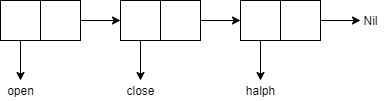
\includegraphics[scale=0.8]{1}
	\centering\caption{'(open close halph)}
\end{figure}

\begin{figure}[h!]
	\centering 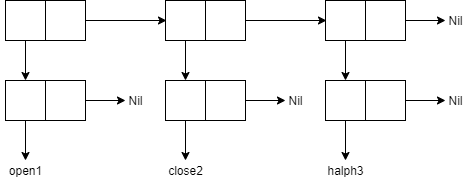
\includegraphics[scale=0.8]{2}
	\centering\caption{'((open1) (close2) (halph3))}
\end{figure}

\begin{figure}[h!]
	\centering 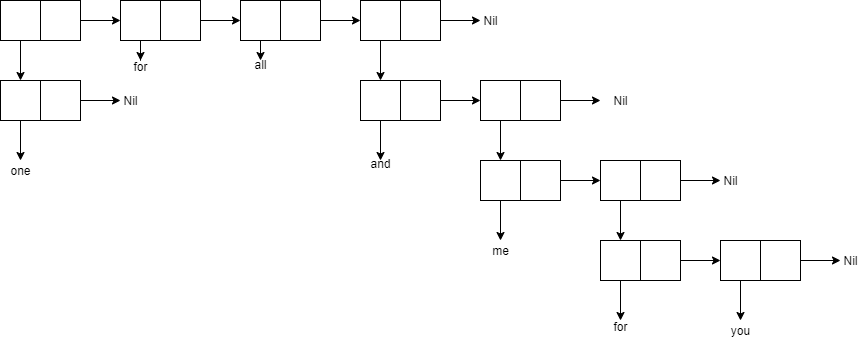
\includegraphics[scale=0.58]{3}
	\centering\caption{'((one) for all (and(me(for you))))}
\end{figure}
\clearpage
\newpage
\begin{figure}[h!]
	\centering 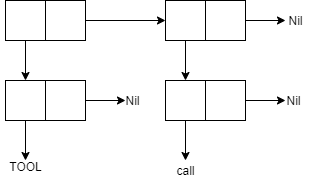
\includegraphics[scale=0.8]{4}
	\centering\caption{'((TOOL) (call))}
\end{figure}
\begin{figure}[h!]
	\centering 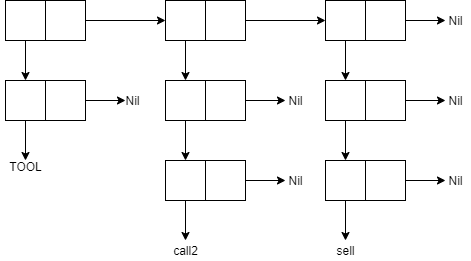
\includegraphics[scale=0.8]{5}
	\centering\caption{'((TOOL1)((call2)) ((sell)))}
\end{figure}
\clearpage
\newpage
\begin{figure}[h!]
	\centering 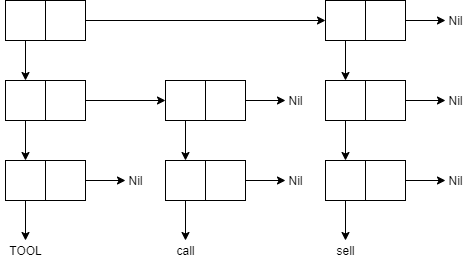
\includegraphics[scale=0.8]{6}
	\centering\caption{'(((TOOL) (call)) ((sell)))}
\end{figure} 

\clearpage
\newpage

\printbibliography
\addcontentsline{toc}{section}{Список литературы}

\end{document}